\RequirePackage{fix-cm}
\documentclass{article}
\usepackage[paperwidth=84.1cm,paperheight=59.4cm,margin=0cm]{geometry}
\usepackage{tikz}
\usetikzlibrary{arrows.meta,backgrounds,calc,positioning}
\usepackage{graphicx}
\usepackage{xcolor}
\usepackage{amsmath}
\usepackage{ragged2e}
\usepackage[hidelinks]{hyperref}
\renewcommand{\familydefault}{\sfdefault}
\pagestyle{empty}

\definecolor{Ink}{HTML}{17212B}
\definecolor{Navy}{HTML}{183B56}
\definecolor{Teal}{HTML}{147D78}
\definecolor{Green}{HTML}{2E7D4F}
\definecolor{Coral}{HTML}{C65353}
\definecolor{Gold}{HTML}{D69A2D}
\definecolor{Paper}{HTML}{F5F7F9}
\definecolor{Line}{HTML}{CCD5DD}
\definecolor{SoftBlue}{HTML}{EAF1F6}
\definecolor{SoftGreen}{HTML}{E8F4ED}
\definecolor{SoftCoral}{HTML}{FAECEC}

\setlength{\parindent}{0pt}
\setlength{\fboxsep}{0pt}

\newcommand{\PosterBox}[6]{%
  \draw[fill=white,draw=Line,line width=1.2pt,rounded corners=0.3cm]
    ([xshift=#1cm,yshift=-#2cm]current page.north west)
    rectangle ++(#3cm,-#4cm);
  \fill[Navy,rounded corners=0.3cm]
    ([xshift=#1cm,yshift=-#2cm]current page.north west)
    rectangle ++(#3cm,-1.65cm);
  \node[anchor=north west,text=white,font=\fontsize{25}{29}\selectfont\bfseries]
    at ($([xshift=#1cm,yshift=-#2cm]current page.north west)+(0.55cm,-0.34cm)$)
    {#5};
  \node[anchor=north west,inner sep=0pt,text=Ink]
    at ($([xshift=#1cm,yshift=-#2cm]current page.north west)+(0.55cm,-2.02cm)$)
    {\begin{minipage}[t]{\dimexpr #3cm-1.10cm\relax}
      \fontsize{17.5}{21}\selectfont\RaggedRight #6
    \end{minipage}};
}

\begin{document}
\begin{tikzpicture}[remember picture,overlay]
  \fill[Paper] (current page.south west) rectangle (current page.north east);

  % Header
  \fill[Navy] (current page.north west) rectangle
    ([yshift=-7.1cm]current page.north east);
  \fill[Teal] ([yshift=-6.78cm]current page.north west) rectangle
    ([yshift=-7.1cm]current page.north east);
  \node[anchor=north west,text=white]
    at ([xshift=1.7cm,yshift=-1.05cm]current page.north west)
    {\fontsize{38}{42}\selectfont\bfseries Beta Function Calculator};
  \node[anchor=north west,text=white]
    at ([xshift=1.75cm,yshift=-3.05cm]current page.north west)
    {\fontsize{22}{26}\selectfont Deliverable 3: Numerical Correctness, Code Quality, Accessibility, and Testing};
  \node[anchor=north east,text=white]
    at ([xshift=-1.8cm,yshift=-0.92cm]current page.north east)
    {\fontsize{19}{22}\selectfont\bfseries Wei Huang};
  \node[anchor=north east,text=white]
    at ([xshift=-1.8cm,yshift=-1.82cm]current page.north east)
    {\fontsize{13.5}{16}\selectfont SOEN 6011 \textbar{} Summer 2026};
  \node[anchor=north east,fill=Gold,text=Ink,rounded corners=0.35cm,
        inner xsep=0.55cm,inner ysep=0.25cm]
    at ([xshift=-1.8cm,yshift=-3.12cm]current page.north east)
    {\fontsize{17}{20}\selectfont\bfseries Semantic Version 1.0.0};
  \node[anchor=south,text=white]
    at ([yshift=0.55cm]current page.north -| current page.center)
    {};
  \node[anchor=center,text=white]
    at ([yshift=-5.25cm]current page.north)
    {\fontsize{25}{29}\selectfont
      $\boldsymbol{B(x,y)}=
       \dfrac{\boldsymbol{\Gamma(x)\Gamma(y)}}{\boldsymbol{\Gamma(x+y)}}\,,
       \qquad \boldsymbol{x>0,\ y>0}$};

  % Left column
  \PosterBox{1.5}{8.0}{26.1}{27.0}{Final Graphical Interface}{
    \centering
    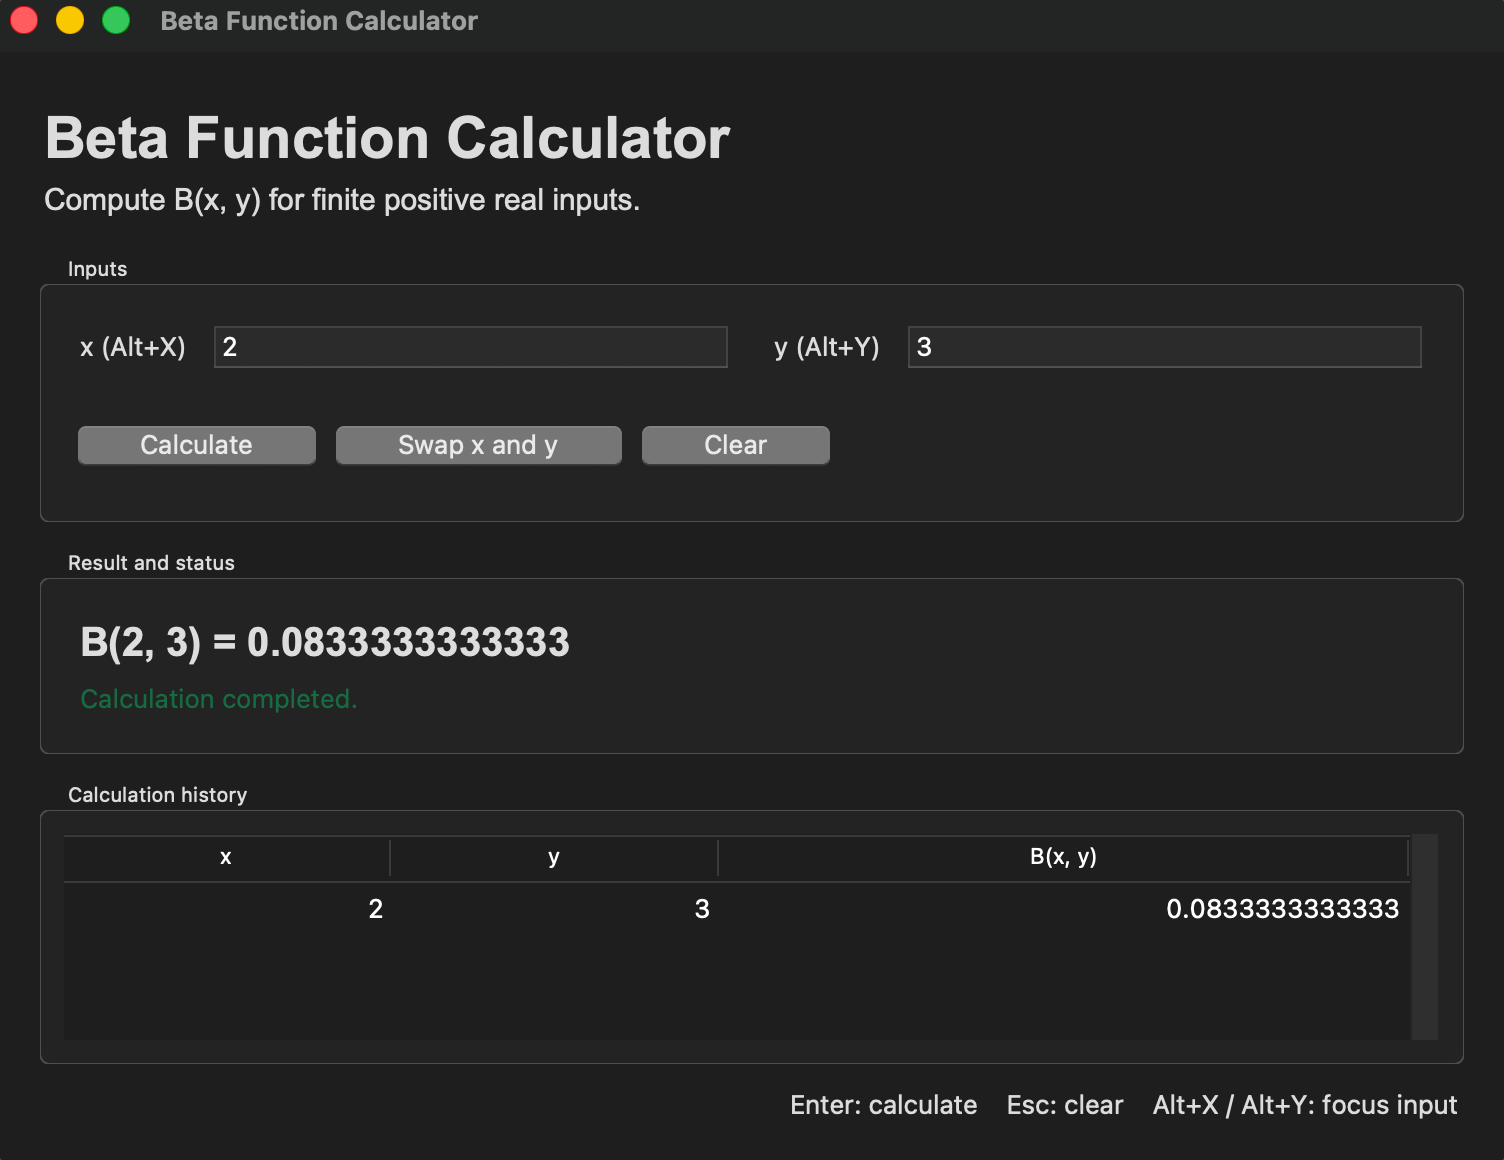
\includegraphics[width=24.8cm]{assets/gui_raw.png}
    \par\vspace{0.35cm}
    \RaggedRight
    The live interface demonstrates a known value, visible calculation status,
    and persistent history. Native Tkinter widgets preserve familiar focus and
    tab behavior.
  }

  \PosterBox{1.5}{35.7}{26.1}{15.4}{Accessibility and Recovery}{
    \begin{tikzpicture}[x=1cm,y=1cm]
      \node[draw=Teal,fill=SoftGreen,rounded corners=0.18cm,
            text width=10.8cm,minimum height=1.65cm,align=center,font=\bfseries]
        at (5.8,0) {Keyboard access\\Enter, Esc, Alt+X, Alt+Y};
      \node[draw=Navy,fill=SoftBlue,rounded corners=0.18cm,
            text width=10.8cm,minimum height=1.65cm,align=center,font=\bfseries]
        at (18.1,0) {Recognition over recall\\visible labels and actions};
      \node[draw=Coral,fill=SoftCoral,rounded corners=0.18cm,
            text width=10.8cm,minimum height=1.65cm,align=center,font=\bfseries]
        at (5.8,-2.15) {Helpful recovery\\field-specific text messages};
      \node[draw=Green,fill=SoftGreen,rounded corners=0.18cm,
            text width=10.8cm,minimum height=1.65cm,align=center,font=\bfseries]
        at (18.1,-2.15) {Status is not color-only\\words identify success or error};
    \end{tikzpicture}
    \vspace{0.25cm}

    The GUI aims to be accessible through readable labels, visible focus,
    redundant text feedback, keyboard operation, and recoverable validation.
    These choices align the interface with the user's task model
    (Kamthan, 2026c).

    \vspace{0.35cm}
    \textbf{Exception policy:} expected input and numeric-range errors receive
    specific messages; unexpected arithmetic failures are not hidden behind a
    generic message and remain available for diagnosis.

    \vspace{0.35cm}
    \textbf{D3 conclusion:} the release improves numerical stability,
    accessibility, and software quality through a stable log-beta
    implementation, explicit range behavior, and repeatable verification.
  }

  % Centre column
  \PosterBox{28.4}{8.0}{26.8}{13.5}{Problem 7: Style and Static Analysis}{
    \centering
    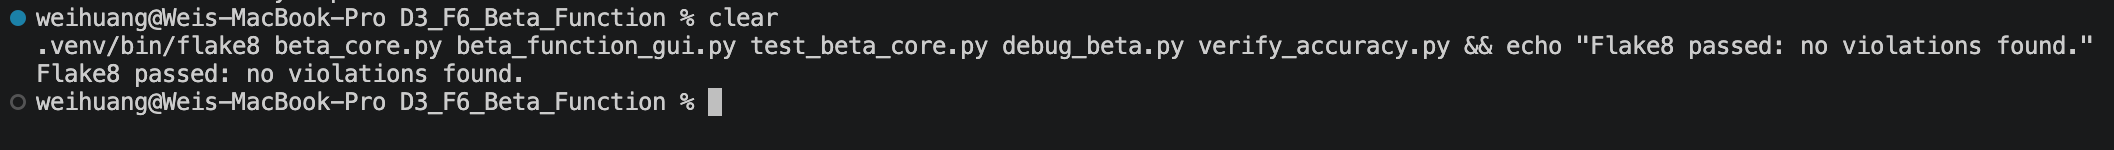
\includegraphics[width=25.2cm]{assets/flake8_raw.png}
    \par\vspace{0.22cm}
    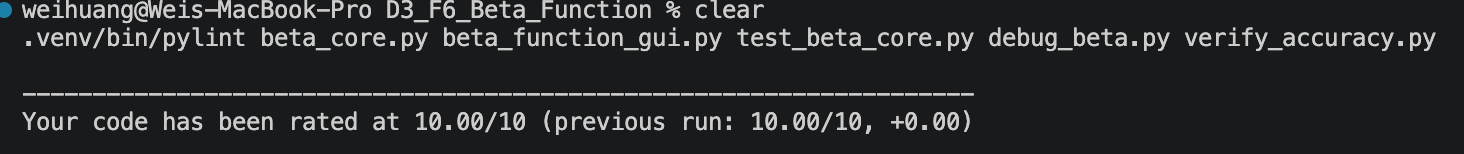
\includegraphics[width=25.2cm]{assets/pylint_raw.png}
    \par\vspace{0.24cm}
    \RaggedRight
    Flake8 reports no PEP 8 style violations; Pylint rates the final source
    \textbf{10.00/10}. Both outputs were generated from version 1.0.0.
  }

  \PosterBox{28.4}{22.2}{26.8}{14.7}{Problem 7: Debugger Evidence}{
    \centering
    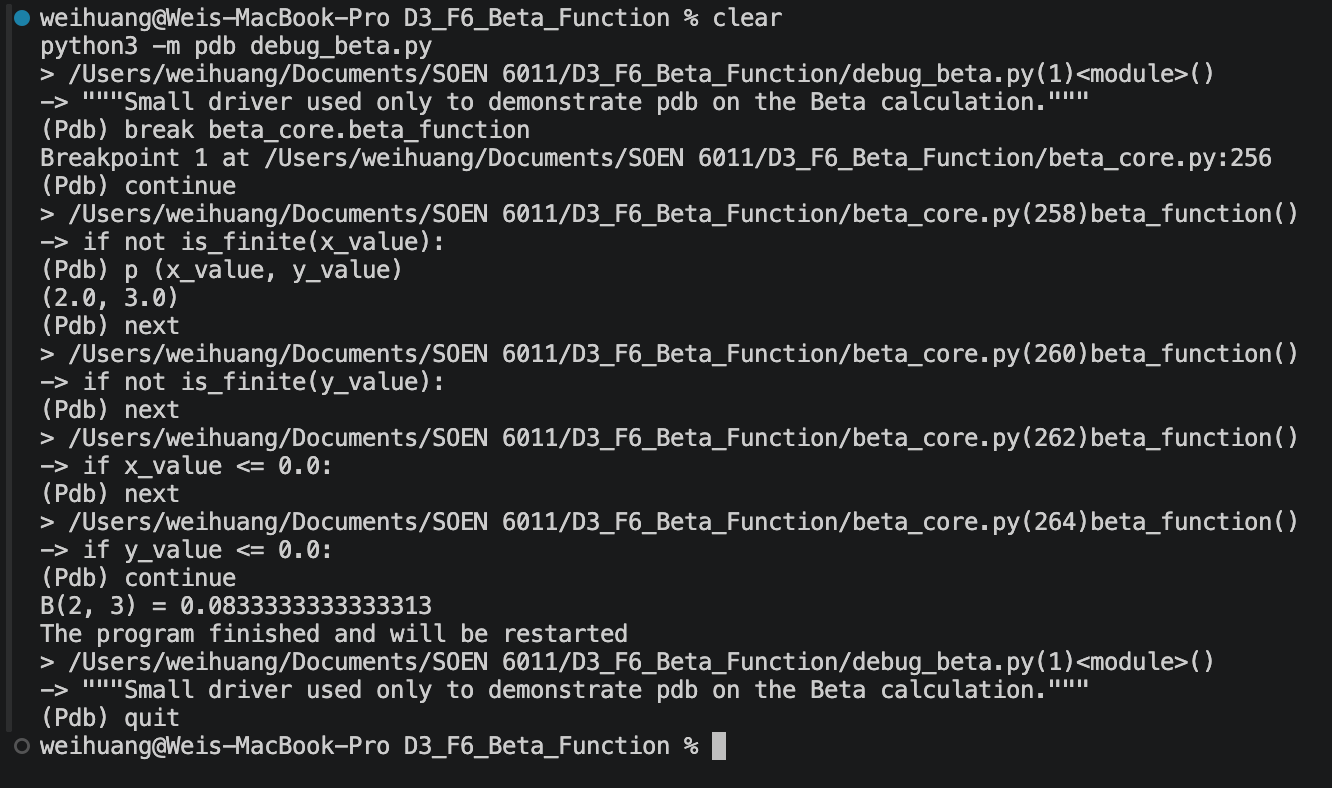
\includegraphics[height=9.7cm]{assets/pdb_raw.png}
    \par\vspace{0.3cm}
    \RaggedRight
    A reproducible \texttt{pdb} session stops inside \texttt{beta\_function},
    inspects $(x,y)=(2,3)$, steps through validation, and confirms the known
    result $1/12$.
  }

  \PosterBox{28.4}{37.6}{26.8}{13.5}{Verified Numerical Contract}{
    \centering
    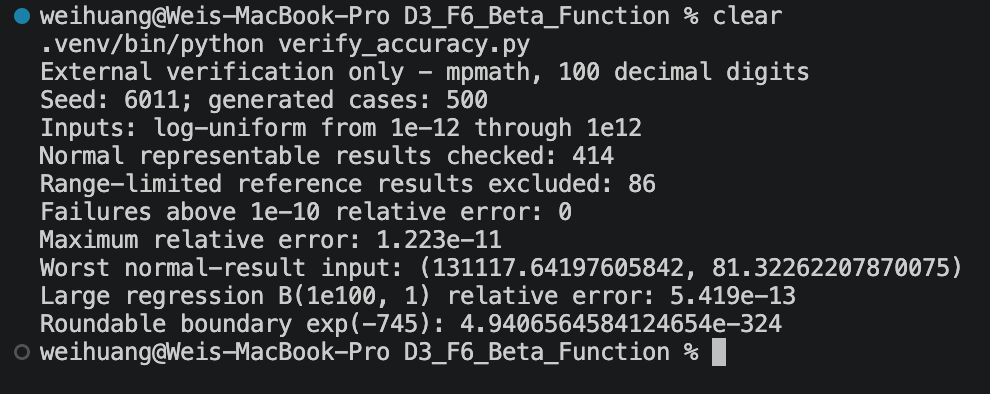
\includegraphics[width=23.5cm]{assets/accuracy_raw.png}
    \par\vspace{0.18cm}
    \fontsize{14}{17}\selectfont\RaggedRight
    \textbf{Contract:} finite positive inputs produce a representable binary64
    result or a specific range error. Twelve displayed digits are formatting,
    not a universal accuracy claim; subnormal values follow binary64 spacing.
  }

  % Right column
  \PosterBox{56.0}{8.0}{26.6}{23.7}{UIDP Decision Mind Map}{
    \centering
    \vspace{0.45cm}
    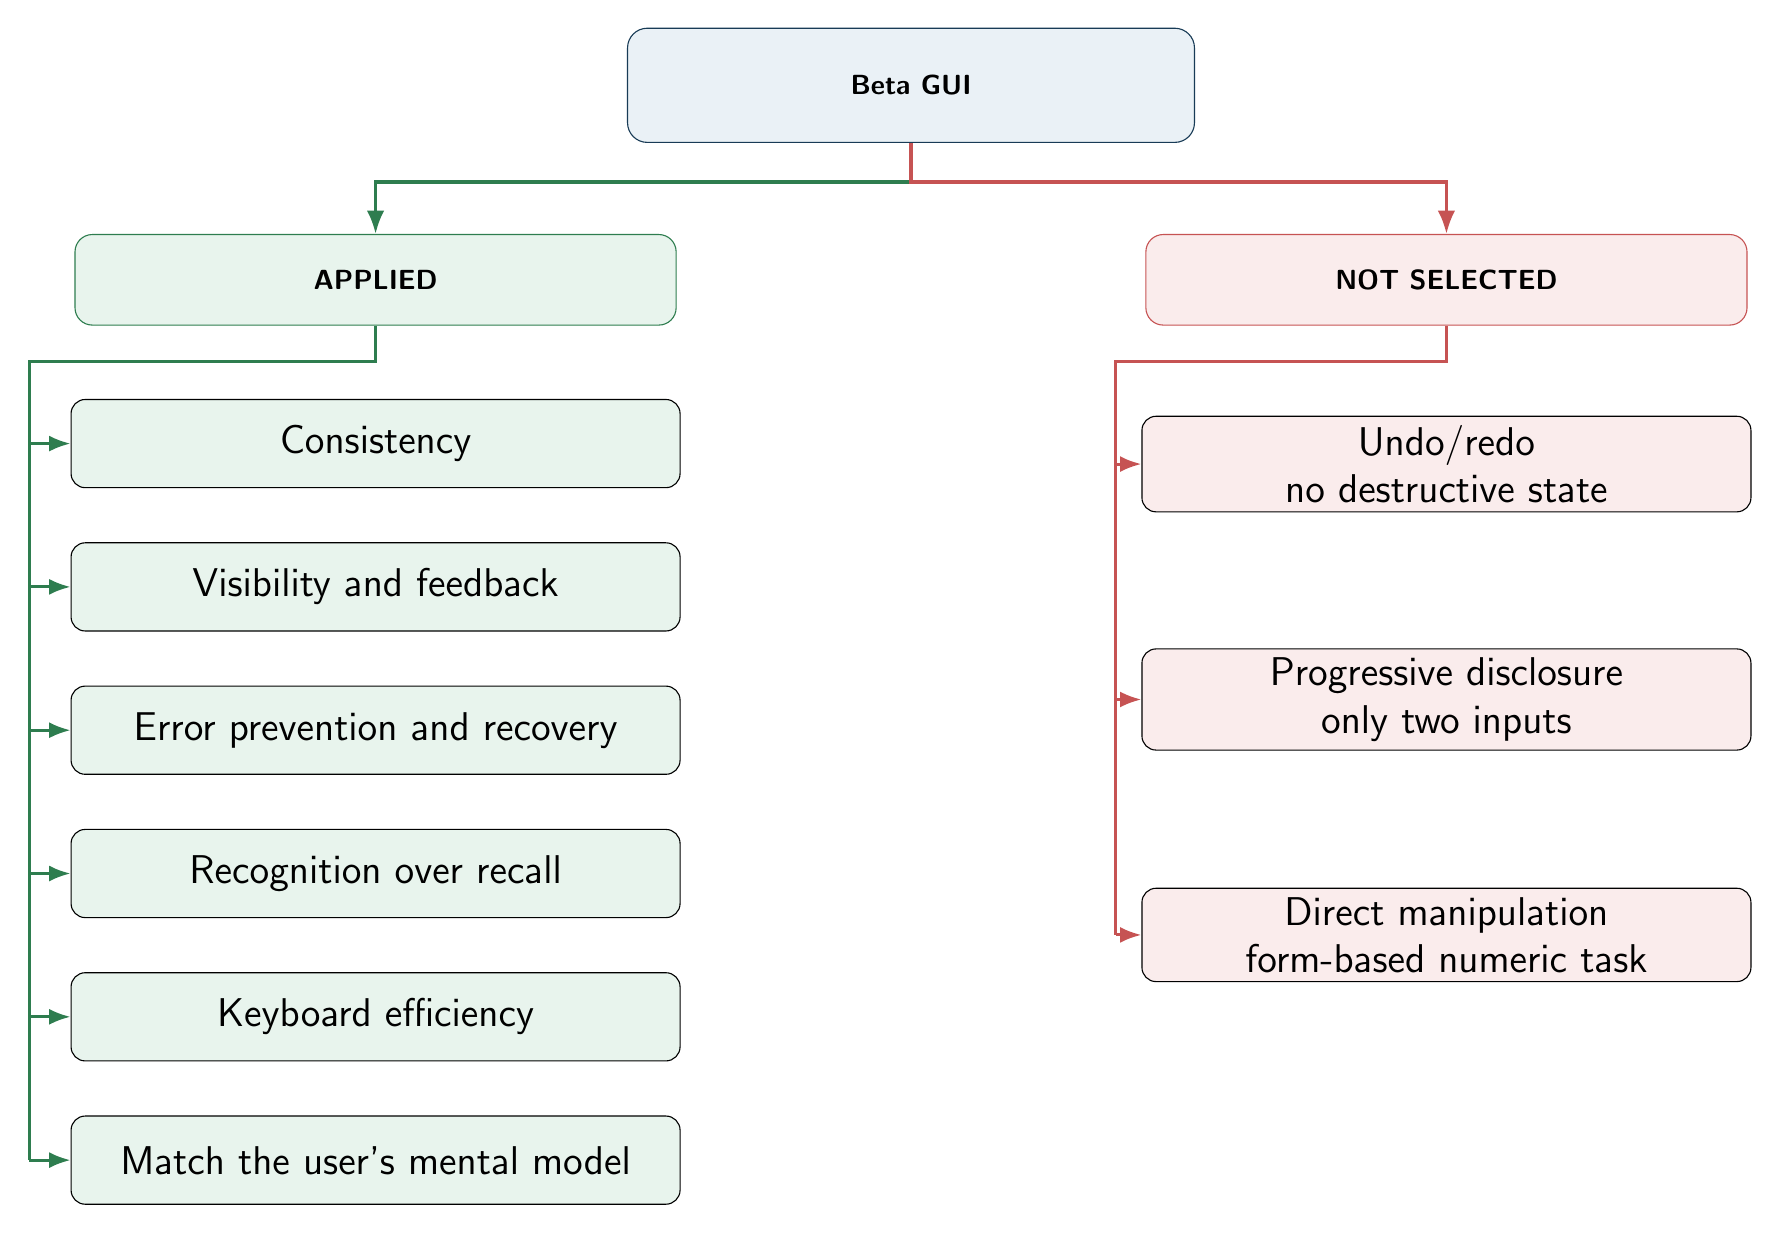
\begin{tikzpicture}[y=1.30cm,
      every node/.style={font=\fontsize{14.5}{17}\selectfont},
      branch/.style={draw,rounded corners=0.18cm,minimum height=1.12cm,
                     text width=7.5cm,align=center},
      >=Latex
    ]
      \node[draw=Navy,fill=SoftBlue,rounded corners=0.25cm,
            minimum width=7.2cm,minimum height=1.45cm,font=\bfseries] (root)
            at (0,1.35) {Beta GUI};
      \node[draw=Green,fill=SoftGreen,rounded corners=0.22cm,
            text width=7.4cm,minimum height=1.15cm,align=center,font=\bfseries] (apply)
            at (-6.8,-0.55) {APPLIED};
      \node[draw=Coral,fill=SoftCoral,rounded corners=0.22cm,
            text width=7.4cm,minimum height=1.15cm,align=center,font=\bfseries] (omit)
            at (6.8,-0.55) {NOT SELECTED};

      \node[branch,fill=SoftGreen] (a1) at (-6.8,-2.15) {Consistency};
      \node[branch,fill=SoftGreen] (a2) at (-6.8,-3.55) {Visibility and feedback};
      \node[branch,fill=SoftGreen] (a3) at (-6.8,-4.95) {Error prevention and recovery};
      \node[branch,fill=SoftGreen] (a4) at (-6.8,-6.35) {Recognition over recall};
      \node[branch,fill=SoftGreen] (a5) at (-6.8,-7.75) {Keyboard efficiency};
      \node[branch,fill=SoftGreen] (a6) at (-6.8,-9.15) {Match the user's mental model};

      \node[branch,fill=SoftCoral] (n1) at (6.8,-2.35)
        {Undo/redo\\no destructive state};
      \node[branch,fill=SoftCoral] (n2) at (6.8,-4.65)
        {Progressive disclosure\\only two inputs};
      \node[branch,fill=SoftCoral] (n3) at (6.8,-6.95)
        {Direct manipulation\\form-based numeric task};

      \begin{scope}[on background layer]
        \draw[->,line width=1.2pt,Green]
          (root.south) -- ++(0,-0.38) -| (apply.north);
        \draw[->,line width=1.2pt,Coral]
          (root.south) -- ++(0,-0.38) -| (omit.north);

        \draw[line width=1.05pt,Green]
          (apply.south) -- ++(0,-0.35) -| (-11.2,-9.15);
        \foreach \nodeName in {a1,a2,a3,a4,a5,a6}
          \draw[->,line width=1.05pt,Green]
            (-11.2,0 |- \nodeName.west) -- (\nodeName.west);

        \draw[line width=1.05pt,Coral]
          (omit.south) -- ++(0,-0.35) -| (2.6,-6.95);
        \foreach \nodeName in {n1,n2,n3}
          \draw[->,line width=1.05pt,Coral]
            (2.6,0 |- \nodeName.west) -- (\nodeName.west);
      \end{scope}
    \end{tikzpicture}
    \vspace{1.0cm}

    The mind map records both selected and rejected principles instead of
    treating every principle as mandatory (Kamthan, 2026d).
  }

  \PosterBox{56.0}{32.4}{26.6}{18.7}{Problem 8: PyUnit Test Suite}{
    \centering
    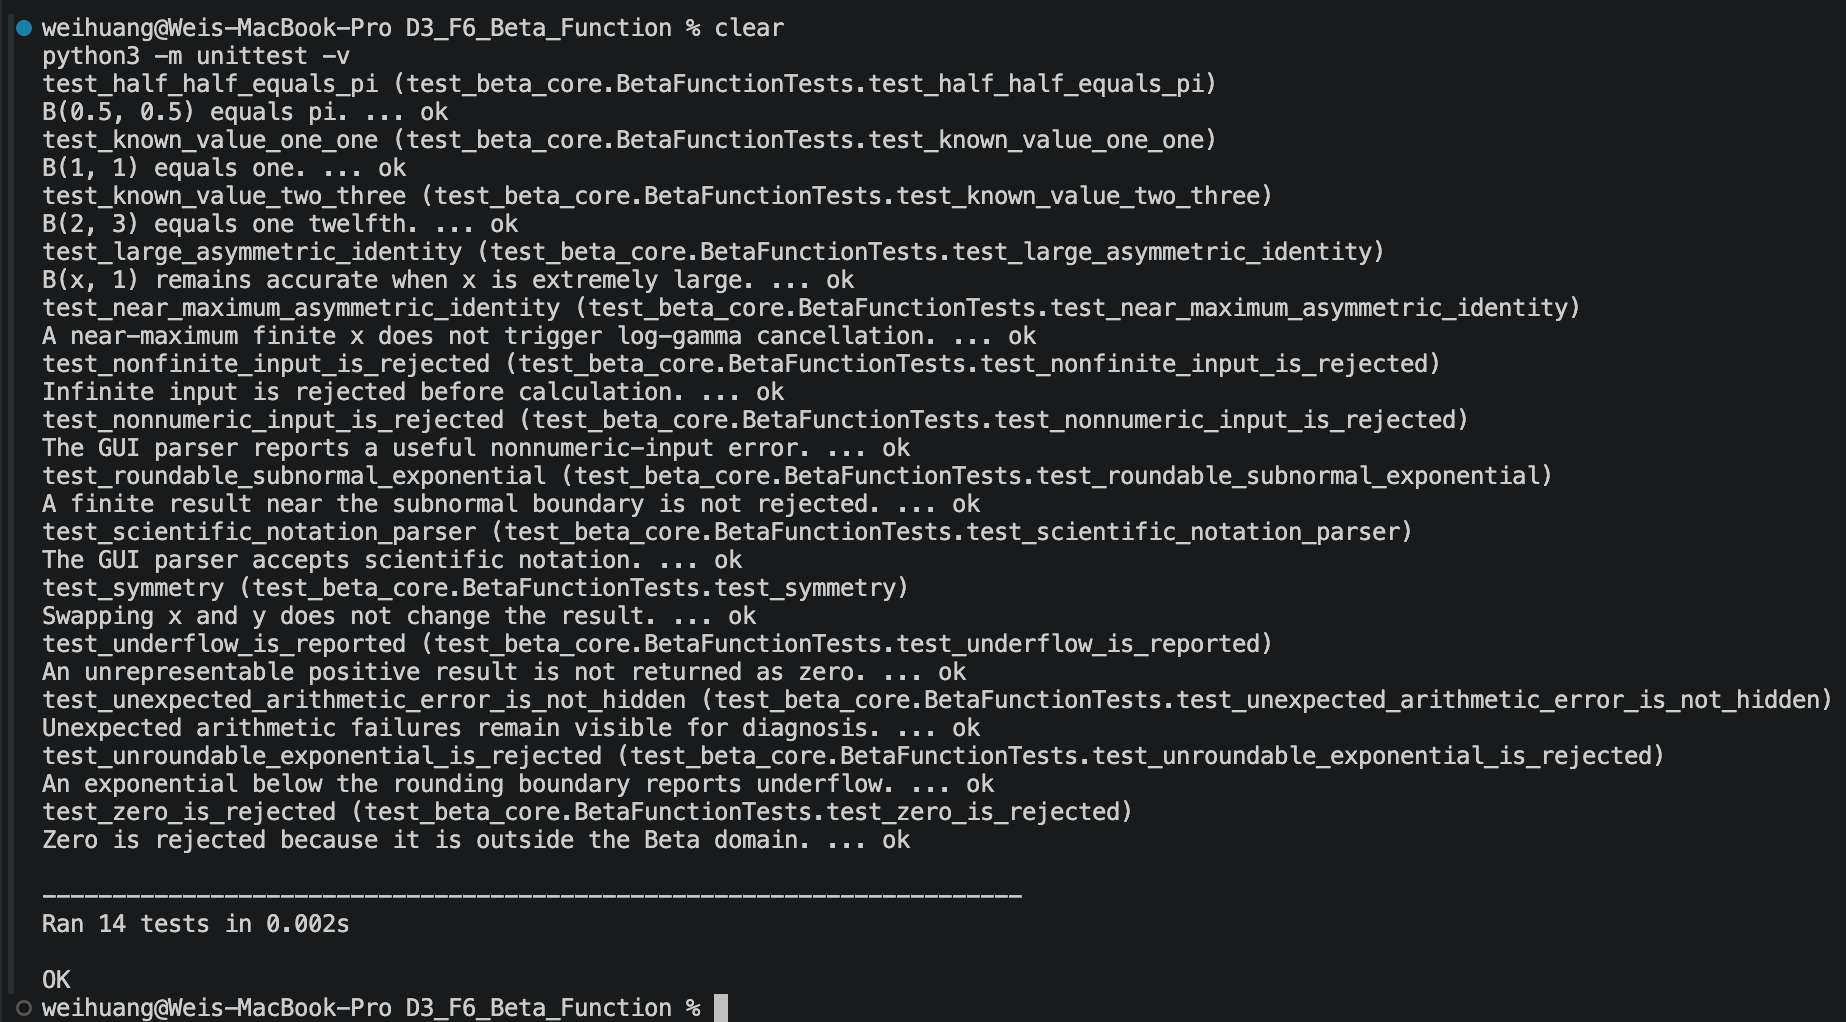
\includegraphics[height=12.5cm]{assets/unit_tests_raw.png}
    \par\vspace{0.25cm}
    \RaggedRight
    \textbf{14/14 tests pass.} Coverage includes trusted values, symmetry,
    extreme asymmetric inputs, the roundable subnormal boundary, scientific
    notation, invalid input, underflow, and propagation of unexpected
    arithmetic errors. The tests exercise the final numerical core and parser.
  }

  % Footer: GAI use and references
  \draw[fill=Ink,draw=Ink]
    ([xshift=1.5cm,yshift=-52.0cm]current page.north west)
    rectangle ([xshift=-1.5cm,yshift=1.1cm]current page.south east);
  \node[anchor=north west,text=white,inner sep=0pt]
    at ([xshift=2.1cm,yshift=-52.55cm]current page.north west)
    {\begin{minipage}[t]{39.2cm}
      \fontsize{15.5}{18.5}\selectfont\RaggedRight
      \textbf{Generative AI and CASTROFF.} Tool: OpenAI ChatGPT/Codex.
      Problem 7 prompt: ``Review the stable log-beta code for PEP 8, Flake8,
      pdb, Pylint, SemVer, UIDP, accessibility, and honest range behavior.''
      Problem 8 prompt: ``Propose PyUnit regressions for large inputs,
      subnormal rounding, invalid input, and unexpected exceptions.''
      Context: SOEN 6011 D3; Audience: TA/instructor; Style: concise; Task:
      review; Role: student engineer; Output: suggestions; Format: poster
      checklist; Feedback: accept only after execution. Suggestions were
      revised and verified; unverified claims were rejected.
    \end{minipage}};
  \node[anchor=north west,text=white,inner sep=0pt]
    at ([xshift=43.1cm,yshift=-52.55cm]current page.north west)
    {\begin{minipage}[t]{38.3cm}
      \fontsize{15.5}{18.5}\selectfont\RaggedRight
      \textbf{References.} Kamthan, P. (2026a), \textit{SOEN 6011 Project
      Description}. Kamthan, P. (2026b), \textit{Building, Versioning, and
      Releasing Software}. Kamthan, P. (2026c), \textit{Introduction to Mental
      Models}. Kamthan, P. (2026d), \textit{Brainstorming and Mind Mapping}.
      Van Rossum, G., Warsaw, B., and Coghlan, N. (2001), \textit{PEP 8 -- Style
      Guide for Python Code}. Python Software Foundation (2026),
      \textit{unittest and pdb Documentation}.

      \vspace{0.35cm}
      \textbf{Repository:}
      \href{https://github.com/HW925/SOEN-6011-D3-Beta-Function}
      {github.com/HW925/SOEN-6011-D3-Beta-Function}
    \end{minipage}};

\end{tikzpicture}
\end{document}
